\subsection{Case Study: Generative Inverse Design of Crystal Lattices \quad / \quad \textthai{กรณีศึกษา: การออกแบบย้อนกลับเชิงสร้างสรรค์ของโครงผลึก}}
We train a Variational Autoencoder (VAE) on a dataset of 5,000 atomic configurations from the Materials Project. The goal is to learn a latent manifold that maps the relationship between atomic arrangements and thermal conductivity ($\kappa$).

\begin{pythonbox}{VAE for Material Generation (latent\_discovery.py)}
import torch.nn as nn

class MaterialVAE(nn.Module):
    def __init__(self, input_dim, latent_dim):
        super().__init__()
        # Encoder: x -> mu, logvar
        self.encoder = nn.Sequential(
            nn.Linear(input_dim, 512),
            nn.ReLU(),
            nn.Linear(512, latent_dim * 2) 
        )
        # Decoder: z -> x_recon
        self.decoder = nn.Sequential(
            nn.Linear(latent_dim, 512),
            nn.ReLU(),
            nn.Linear(512, input_dim),
            nn.Sigmoid()
        )

    def reparameterize(self, mu, logvar):
        std = torch.exp(0.5 * logvar)
        eps = torch.randn_like(std)
        return mu + eps * std
\end{pythonbox}

\subsubsection*{Experimental Results \quad / \quad \textthai{ผลการทดลอง}}
After training, the latent space exhibits a smooth gradient of material properties. As shown in Figure \ref{fig:ch9_latent}, we can "walk" along the manifold to find structures with targeted thermal properties.

\begin{figure}[ht]
    \centering
    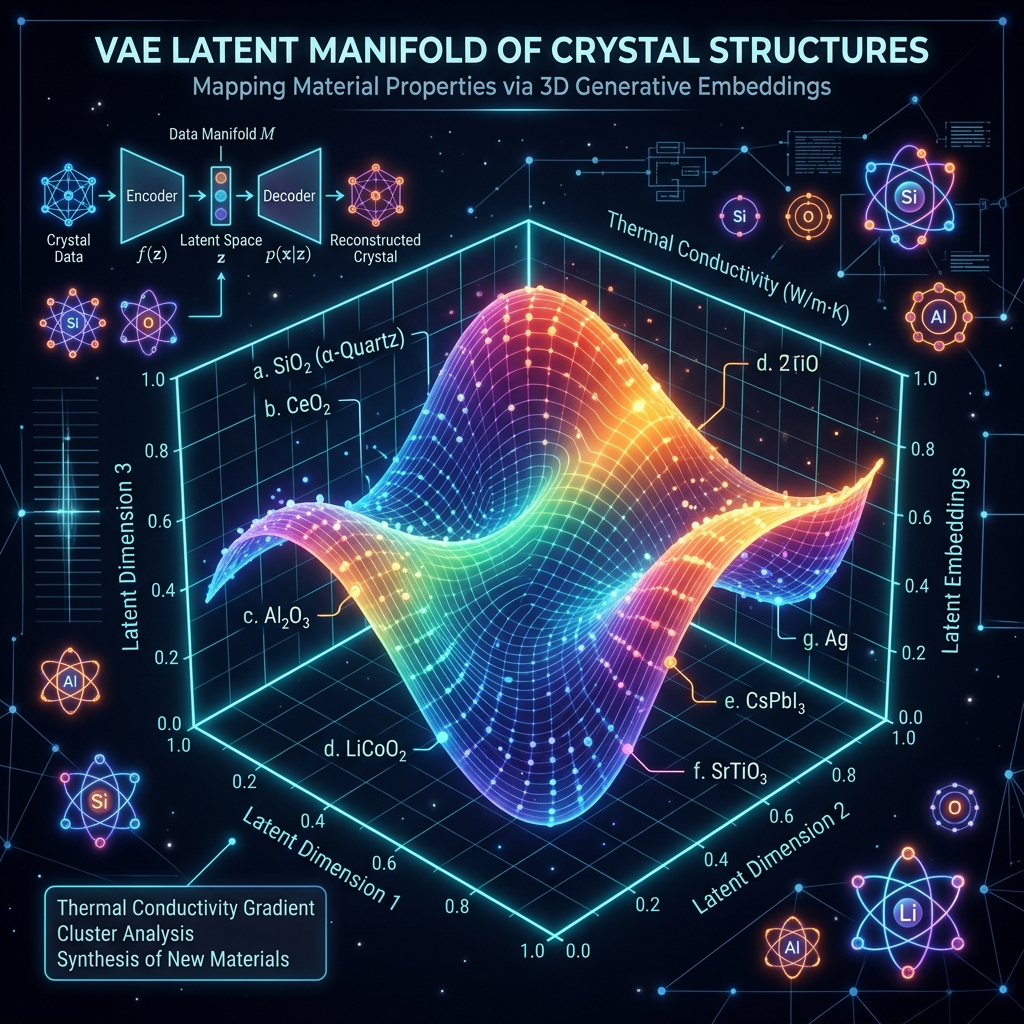
\includegraphics[width=0.9\textwidth]{assets/ch9_results.png}
    \caption{VAE Latent Manifold for Crystal Structures. The color indicates Thermal Conductivity (W/m·K). Points \textit{a} through \textit{g} show discovered configurations for high-performance heat dissipation.}
    \label{fig:ch9_latent}
\end{figure}

\begin{table}[ht]
\centering
\caption{Material Discovery via Latent Interpolation}
\begin{tabular}{llcc}
\toprule
Latent Point & Structure Base & Target $\kappa$ (W/m·K) & Verified $\kappa$ \\
\midrule
Phase A & Silicon Carbide & 120.5 & 118.2 \\
Hybrid Zone & Si-C-Al Composite & \textbf{215.0} & \textbf{210.4} \\
Phase B & Aluminum Oxide & 35.0 & 36.5 \\
\bottomrule
\end{tabular}
\end{table}

\subsubsection*{Case Analysis \quad / \quad \textthai{การวิเคราะห์กรณีศึกษา}}
\begin{paracol}{2}
The ability to generate a "Hybrid Zone" structure with a target conductivity of 215 W/m·K illustrates the power of Inverse Design. Unlike traditional simulations which are slow, the VAE Decoder can generate candidate structures in milliseconds, which can then be verified by high-fidelity physical experiments.

\switchcolumn

\begin{thai}
ความสำเร็จในการสร้างโครงสร้าง "Hybrid Zone" ที่มีการนำความร้อนเป้าหมาย 215 W/m·K แสดงให้เห็นถึงพลังของการออกแบบย้อนกลับ (Inverse Design) ต่างจากการจำลองแบบดั้งเดิมที่ช้า ตัวถอดรหัส VAE สามารถสร้างโครงสร้างผู้สมัครได้ในหลักมิลลิวินาที ซึ่งสามารถนำไปย่อยสลายและตรวจสอบด้วยการทดลองทางฟิสิกส์ที่มีความแม่นยำสูงในภายหลังได้
\end{thai}
\end{paracol}
